\documentclass[12pt,a4paper]{article}

% ── Packages ──────────────────────────────────────────────────────────
\usepackage[margin=1in]{geometry}
\usepackage{graphicx}
\usepackage{xcolor}
\usepackage{tikz}
\usepackage{booktabs}
\usepackage{tabularx}
\usepackage{longtable}
\usepackage{enumitem}
\usepackage{listings}
\usepackage{fancyhdr}
\usepackage{hyperref}
\usepackage{titlesec}
\usepackage{tcolorbox}
\usepackage{fontenc}
\usepackage[T1]{fontenc}
\usepackage{lmodern}
\usepackage{parskip}
\usepackage{multicol}
\usepackage{float}
\usepackage{amssymb}  % for \checkmark
\usepackage{array}

\tcbuselibrary{skins,breakable}

% ── Colors ────────────────────────────────────────────────────────────
\definecolor{emisblue}{RGB}{0,71,133}
\definecolor{emisdark}{RGB}{20,40,70}
\definecolor{emislight}{RGB}{230,240,250}
\definecolor{accentgreen}{RGB}{40,160,80}
\definecolor{accentorange}{RGB}{220,120,20}
\definecolor{codebg}{RGB}{245,245,245}
\definecolor{codeborder}{RGB}{200,200,200}
\definecolor{warnbg}{RGB}{255,248,230}
\definecolor{warnborder}{RGB}{220,180,50}
\definecolor{tipbg}{RGB}{230,248,235}
\definecolor{tipborder}{RGB}{40,160,80}

% ── Hyperref ──────────────────────────────────────────────────────────
\hypersetup{
    colorlinks=true,
    linkcolor=emisblue,
    urlcolor=emisblue,
    pdfauthor={EMIS IT Department},
    pdftitle={Active Directory Lab Setup Guide},
    pdfsubject={Windows Server AD DS with RBAC},
}

% ── Code Listings ─────────────────────────────────────────────────────
\lstdefinestyle{powershell}{
    backgroundcolor=\color{codebg},
    basicstyle=\ttfamily\small,
    breaklines=true,
    frame=single,
    rulecolor=\color{codeborder},
    framesep=6pt,
    xleftmargin=6pt,
    xrightmargin=6pt,
    showstringspaces=false,
    tabsize=4,
    keywordstyle=\color{emisblue}\bfseries,
    commentstyle=\color{gray},
    stringstyle=\color{accentgreen},
    numbers=none,
    literate={→}{$\rightarrow$}1 {←}{$\leftarrow$}1,
}
\lstset{style=powershell}

% ── Custom Boxes ──────────────────────────────────────────────────────
\newtcolorbox{warningbox}{
    colback=warnbg, colframe=warnborder,
    arc=2pt, boxrule=1pt,
    left=8pt, right=8pt, top=6pt, bottom=6pt,
    fonttitle=\bfseries,
    title={\textcolor{accentorange}{$\triangle$ Important}},
    breakable
}

\newtcolorbox{tipbox}{
    colback=tipbg, colframe=tipborder,
    arc=2pt, boxrule=1pt,
    left=8pt, right=8pt, top=6pt, bottom=6pt,
    fonttitle=\bfseries,
    title={\textcolor{accentgreen}{\checkmark\ Tip}},
    breakable
}

\newtcolorbox{cmdbox}[1][]{
    colback=codebg, colframe=codeborder,
    arc=2pt, boxrule=0.8pt,
    left=8pt, right=8pt, top=6pt, bottom=6pt,
    breakable, #1
}

% ── Section Styling ───────────────────────────────────────────────────
\titleformat{\section}
    {\Large\bfseries\color{emisblue}}
    {Part \thesection:}{0.5em}{}
    [\vspace{-4pt}\textcolor{emisblue}{\rule{\textwidth}{1.5pt}}]

\titleformat{\subsection}
    {\large\bfseries\color{emisdark}}
    {\thesubsection}{0.5em}{}

\titleformat{\subsubsection}
    {\normalsize\bfseries\color{emisdark}}
    {\thesubsubsection}{0.5em}{}

% ── Header / Footer ──────────────────────────────────────────────────
\pagestyle{fancy}
\fancyhf{}
\fancyhead[L]{\small\textcolor{gray}{EMIS --- Active Directory Lab Guide}}
\fancyhead[R]{\small\textcolor{gray}{Confidential}}
\fancyfoot[C]{\small\textcolor{gray}{Page \thepage}}
\fancyfoot[R]{\small\textcolor{gray}{June 2026}}
\renewcommand{\headrulewidth}{0.4pt}
\renewcommand{\footrulewidth}{0.2pt}

% ══════════════════════════════════════════════════════════════════════
\begin{document}

% ── Title Page ────────────────────────────────────────────────────────
\begin{titlepage}
\begin{tikzpicture}[remember picture, overlay]
    % Top blue bar
    \fill[emisblue] (current page.north west) rectangle ([yshift=-4cm]current page.north east);
    % Accent line
    \fill[accentgreen] ([yshift=-4cm]current page.north west) rectangle ([yshift=-4.15cm]current page.north east);
    % Bottom bar
    \fill[emisdark] (current page.south west) rectangle ([yshift=2cm]current page.south east);
\end{tikzpicture}

\vspace*{1cm}
\begin{center}
    {\Huge\bfseries\textcolor{white}{Active Directory Lab}}\\[6pt]
    {\Huge\bfseries\textcolor{white}{Setup Guide}}\\[30pt]
\end{center}

\vspace{3cm}

\begin{center}
    {\LARGE\bfseries\textcolor{emisblue}{Windows Server 2019}}\\[10pt]
    {\LARGE\textcolor{emisdark}{Domain Controller with RBAC}}\\[8pt]
    {\large\textcolor{emisdark}{2000 Users --- 5 Labs $\times$ 24 PCs --- Lab Management API}}\\[40pt]

    \textcolor{emisblue}{\rule{0.6\textwidth}{1pt}}\\[20pt]

    {\large
    \begin{tabular}{rl}
        \textbf{Domain:}       & \texttt{emis.local} \\[4pt]
        \textbf{Environment:}  & VMware ESXi 8.0 \\[4pt]
        \textbf{Prepared by:}  & EMIS IT Department \\[4pt]
        \textbf{Date:}         & June 2026 \\[4pt]
        \textbf{Scripts:}       & 4 (AD DS, RBAC, Users, Lab API) \\[4pt]
        \textbf{Version:}      & 2.0 \\
    \end{tabular}
    }
\end{center}

\vfill
\begin{center}
    \textcolor{white}{\small Thapathali Campus --- Institute of Engineering --- Tribhuvan University}
\end{center}
\end{titlepage}

% ── Table of Contents ─────────────────────────────────────────────────
\newpage
\tableofcontents
\newpage

% ══════════════════════════════════════════════════════════════════════
\section{VM Sizing for Domain Controller}
% ══════════════════════════════════════════════════════════════════════

\begin{tipbox}
ESXi is assumed to be already installed and accessible via the web UI.
\end{tipbox}

\begin{table}[H]
\centering
\begin{tabularx}{0.7\textwidth}{l X}
\toprule
\textbf{Resource} & \textbf{Value} \\
\midrule
vCPUs       & 2 \\
RAM         & 4 GB (8 GB recommended) \\
Disk        & 60 GB thin provisioned \\
Network     & 1 vNIC (VM Network) \\
Guest OS    & Windows Server 2019 Standard \\
\bottomrule
\end{tabularx}
\caption{Domain Controller VM Specifications}
\end{table}

% ══════════════════════════════════════════════════════════════════════
\section{Download Windows Server 2019 ISO}
% ══════════════════════════════════════════════════════════════════════

\begin{itemize}
    \item \textbf{Evaluation (180-day free trial):}
    \item \url{https://www.microsoft.com/en-us/evalcenter/evaluate-windows-server-2019}
    \item Choose \textbf{ISO} download, 64-bit edition ($\sim$5.5 GB)
\end{itemize}

% ══════════════════════════════════════════════════════════════════════
\section{Upload ISO and Create VM}
% ══════════════════════════════════════════════════════════════════════

\subsection{Upload Windows Server ISO}

\begin{enumerate}
    \item In ESXi web UI $\rightarrow$ \textbf{Storage} $\rightarrow$ \textbf{Datastore browser}
    \item Click \textbf{Create directory} $\rightarrow$ name it \texttt{ISOs}
    \item Click \textbf{Upload} $\rightarrow$ select your Windows Server 2019 ISO
    \item Wait for upload to complete ($\sim$5.5 GB)
\end{enumerate}

\subsection{Create the Virtual Machine}

\begin{enumerate}
    \item \textbf{Virtual Machines} $\rightarrow$ \textbf{Create / Register VM}
    \item Select \textbf{Create a new virtual machine} $\rightarrow$ Next
    \item Configure:
\end{enumerate}

\begin{table}[H]
\centering
\begin{tabularx}{0.85\textwidth}{l X}
\toprule
\textbf{Setting} & \textbf{Value} \\
\midrule
Name               & \texttt{WinServer-DC} \\
Guest OS family    & Windows \\
Guest OS version   & Microsoft Windows Server 2019 (64-bit) \\
CPU                & 2 \\
Memory             & 4096 MB (4 GB) \\
Hard disk 1        & 60 GB (Thin Provisioned) \\
Network Adapter    & VM Network, VMXNET3 \\
CD/DVD Drive       & Datastore ISO file $\rightarrow$ Windows Server ISO \\
\bottomrule
\end{tabularx}
\caption{VM Configuration}
\end{table}

\begin{warningbox}
Check \textbf{``Connect at power on''} for the CD/DVD drive, otherwise the VM will not boot from the ISO.
\end{warningbox}

% ══════════════════════════════════════════════════════════════════════
\section{Install Windows Server 2019}
% ══════════════════════════════════════════════════════════════════════

\subsection{Boot and Install}

\begin{enumerate}
    \item Power on the VM and open the console
    \item Press any key when prompted to boot from CD/DVD
    \item Set language, time, and keyboard $\rightarrow$ Click \textbf{Next} $\rightarrow$ \textbf{Install now}
    \item Select: \textbf{Windows Server 2019 Standard (Desktop Experience)}
\end{enumerate}

\begin{warningbox}
Always choose \textbf{Desktop Experience}. ``Server Core'' has no GUI and is command-line only.
\end{warningbox}

\begin{enumerate}[resume]
    \item Accept license terms $\rightarrow$ Next
    \item Select \textbf{Custom: Install Windows only (advanced)}
    \item Select \textbf{Drive 0 Unallocated Space} (60 GB) $\rightarrow$ Next
    \item Wait 10--20 minutes for installation. VM reboots automatically.
    \item Set \textbf{Administrator password} (e.g., \texttt{P@ssw0rd2024!})
\end{enumerate}

\subsection{Configure Networking}

\begin{enumerate}
    \item Open \textbf{Network and Sharing Center} $\rightarrow$ \textbf{Change adapter settings}
    \item Right-click \textbf{Ethernet0} $\rightarrow$ \textbf{Properties}
    \item Select \textbf{Internet Protocol Version 4 (TCP/IPv4)} $\rightarrow$ Properties:
\end{enumerate}

\begin{table}[H]
\centering
\begin{tabularx}{0.6\textwidth}{l X}
\toprule
\textbf{Setting} & \textbf{Value} \\
\midrule
IP address       & \texttt{192.168.1.10} \\
Subnet mask      & \texttt{255.255.255.0} \\
Default gateway  & \texttt{192.168.1.1} \\
Preferred DNS    & \texttt{127.0.0.1} \\
Alternate DNS    & \texttt{8.8.8.8} \\
\bottomrule
\end{tabularx}
\caption{Domain Controller IP Configuration}
\end{table}

\begin{tipbox}
The Preferred DNS is set to \texttt{127.0.0.1} because this server will become the DNS server after AD DS promotion.
\end{tipbox}

\subsection{Set Computer Name}

Open \textbf{PowerShell as Administrator} and run:

\begin{lstlisting}
Rename-Computer -NewName "DC01" -Restart
\end{lstlisting}

Server reboots. Login again after reboot.

% ══════════════════════════════════════════════════════════════════════
\section{Install Active Directory Domain Services}
% ══════════════════════════════════════════════════════════════════════

\subsection{Copy Scripts to the Server}

\textbf{Option A --- USB/Shared folder:}\\
Copy the \texttt{ActiveDirectory} folder to \texttt{C:\textbackslash Scripts\textbackslash} on the server.

\textbf{Option B --- Download from GitHub:}

\begin{lstlisting}
Set-ExecutionPolicy RemoteSigned -Force

New-Item -Path "C:\Scripts" -ItemType Directory -Force

Invoke-WebRequest -Uri "https://raw.githubusercontent.com/sumanmhz/sumanmhz/main/ActiveDirectory/01-Install-AD-DS.ps1" -OutFile "C:\Scripts\01-Install-AD-DS.ps1"

Invoke-WebRequest -Uri "https://raw.githubusercontent.com/sumanmhz/sumanmhz/main/ActiveDirectory/02-Create-RBAC-Structure.ps1" -OutFile "C:\Scripts\02-Create-RBAC-Structure.ps1"

Invoke-WebRequest -Uri "https://raw.githubusercontent.com/sumanmhz/sumanmhz/main/ActiveDirectory/03-Bulk-Create-Users.ps1" -OutFile "C:\Scripts\03-Bulk-Create-Users.ps1"

Invoke-WebRequest -Uri "https://raw.githubusercontent.com/sumanmhz/sumanmhz/main/ActiveDirectory/04-AD-User-API.ps1" -OutFile "C:\Scripts\04-AD-User-API.ps1"
\end{lstlisting}

\subsection{Step 1: Install AD DS and Promote to DC}

\begin{lstlisting}
cd C:\Scripts
.\01-Install-AD-DS.ps1
\end{lstlisting}

This script:
\begin{itemize}
    \item Installs AD-DS, DNS, and GPMC server roles
    \item Promotes the server to a Domain Controller
    \item Creates the forest: \texttt{emis.local} (NetBIOS: \texttt{EMIS})
    \item \textbf{Server reboots automatically} --- wait 2--3 minutes
\end{itemize}

\begin{warningbox}
After reboot, the login screen will show \texttt{EMIS\textbackslash Administrator}. Use your Administrator password to login.
\end{warningbox}

\subsection{Step 2: Create RBAC Structure}

\begin{lstlisting}
cd C:\Scripts
.\02-Create-RBAC-Structure.ps1
\end{lstlisting}

This script creates the complete RBAC framework:

\begin{table}[H]
\centering
\begin{tabularx}{\textwidth}{l l X}
\toprule
\textbf{Component} & \textbf{Count} & \textbf{Details} \\
\midrule
Top-level OUs        & 5  & Users, Groups, Computers, Service Accounts, Disabled \\
Department OUs       & 10 & IT, Admin, Faculty, Students, Finance, HR, Library, Research, Engineering, Management \\
Student sub-OUs      & 5  & Batch-2080 through Batch-2084 \\
Faculty sub-OUs      & 4  & Computer, Electronics, Civil, Electrical Engineering \\
Role Groups          & 3  & Global scope: Role-SuperAdmin, Role-Teacher, Role-Students \\
Resource Groups      & 11 & DomainLocal scope (e.g., Access-WiFi, Access-LMS) \\
GPOs                 & 4  & Password policy, desktop config, lab computers, audit \\
\bottomrule
\end{tabularx}
\caption{RBAC Structure Summary}
\end{table}

\subsubsection{RBAC Model}

The access model follows industry best practice:

\begin{center}
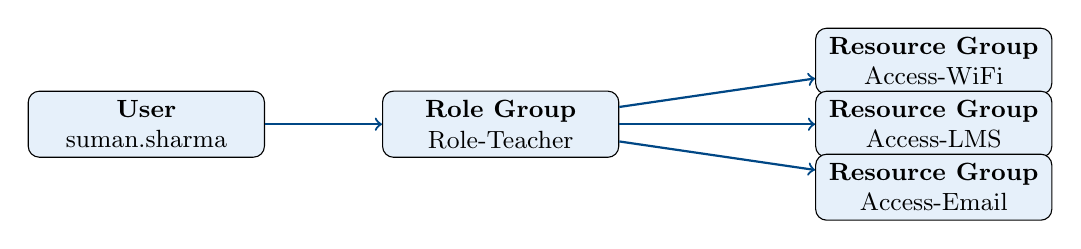
\begin{tikzpicture}[
    box/.style={draw, rounded corners=4pt, fill=emislight, minimum width=3cm, minimum height=0.8cm, align=center, font=\small},
    arrow/.style={->, thick, color=emisblue}
]
    \node[box] (user) at (0,0) {\textbf{User}\\suman.sharma};
    \node[box] (role) at (4.5,0) {\textbf{Role Group}\\Role-Teacher};
    \node[box] (res1) at (10,0.8) {\textbf{Resource Group}\\Access-WiFi};
    \node[box] (res2) at (10,0) {\textbf{Resource Group}\\Access-LMS};
    \node[box] (res3) at (10,-0.8) {\textbf{Resource Group}\\Access-Email};

    \draw[arrow] (user) -- (role);
    \draw[arrow] (role) -- (res1);
    \draw[arrow] (role) -- (res2);
    \draw[arrow] (role) -- (res3);
\end{tikzpicture}
\end{center}

\begin{center}
\texttt{User $\rightarrow$ Role Group $\rightarrow$ Resource Group $\rightarrow$ Actual Permission}
\end{center}

\subsubsection{Role-to-Resource Mappings}

All roles receive the same daily-use resources. Users experience the system normally --- login with their AD username and password, access files, print, browse the internet, use email and LMS. No role feels ``locked down.'' Only infrastructure access (server room, VPN, ERP) is limited to the superadmin role.

\begin{longtable}{l p{10cm}}
\toprule
\textbf{Role Group} & \textbf{Resource Access} \\
\midrule
\endhead
Role-SuperAdmin & FileServer-RW, PrinterColor, PrinterBW, WiFi, VPN, ServerRoom, ERP, LMS, Email, InternetFull, LabComputers \\
Role-Teacher & FileServer-RW, PrinterColor, PrinterBW, WiFi, LMS, Email, InternetFull, LabComputers \\
Role-Students & FileServer-RW, PrinterColor, PrinterBW, WiFi, LMS, Email, InternetFull, LabComputers \\
\bottomrule
\caption{Role-Based Access Control Mappings}
\end{longtable}

\begin{tipbox}
Teachers and students get the \textbf{exact same} resources. The only difference is what they can do through the \textbf{API} --- teachers can monitor labs and reset passwords. On a PC, a student's experience is identical to a teacher's.
\end{tipbox}

\subsection{Step 3: Bulk Create 2000 Users}

\begin{lstlisting}
cd C:\Scripts
.\03-Bulk-Create-Users.ps1 -GenerateSample
\end{lstlisting}

\begin{itemize}
    \item Enter a default password when prompted (e.g., \texttt{Welcome@123})
    \item Generates 2000 users automatically:
    \begin{itemize}
        \item 1400 students (distributed across batches)
        \item 600 staff (across all departments)
    \end{itemize}
    \item Each user is placed in the correct OU by department
    \item Each user is assigned their RBAC role group
    \item Password change is forced at first logon
\end{itemize}

\begin{tipbox}
To use your own user list instead of generated data, create a CSV file with columns: \texttt{FirstName, LastName, Username, Email, Department, Title, Role, Phone} and run:\\[4pt]
\texttt{.\textbackslash 03-Bulk-Create-Users.ps1 -CsvPath "C:\textbackslash myusers.csv"}
\end{tipbox}

% ══════════════════════════════════════════════════════════════════════
\section{Lab \& User Management API (Step 4)}
% ══════════════════════════════════════════════════════════════════════

The API provides centralized management of AD users and lab PCs over REST. It uses \textbf{Pode} (pure PowerShell web framework) and \textbf{WinRM} (PowerShell Remoting) to control domain-joined PCs.

\subsection{Three Roles}

\begin{table}[H]
\centering
\begin{tabularx}{\textwidth}{l l X}
\toprule
\textbf{Role} & \textbf{Who} & \textbf{Permissions} \\
\midrule
\texttt{superadmin} & IT Admin & Full control: CRUD users, bulk create/delete by batch or faculty, shutdown/restart/install software on any PC in any lab \\
\texttt{teacher} & Teacher / TA & Monitor \textbf{any} lab (who's logged in, CPU/RAM, running apps), list students, reset student passwords. Teachers are not assigned to a fixed lab --- they can walk into any lab and access its data. \\
\texttt{student} & Student & Change own password only \\
\bottomrule
\end{tabularx}
\caption{API Role Definitions}
\end{table}

\subsection{Configure Labs}

On first run, the script generates a template \texttt{labs.json}. Edit it to match your actual lab layout:

\begin{lstlisting}
[
  {
    "Name": "Lab-1",
    "Location": "Block A, Room 101",
    "Switch": "10.10.1.1",
    "Subnet": "10.10.1.0/24",
    "Gateway": "10.10.1.1",
    "PCs": [
      { "Hostname": "LAB1-PC01", "IP": "10.10.1.11" },
      { "Hostname": "LAB1-PC02", "IP": "10.10.1.12" }
    ]
  }
]
\end{lstlisting}

Each lab has its own switch and subnet. PCs within a lab are interconnected through that switch.

\subsection{Generate Service Keys}

\begin{lstlisting}
cd C:\Scripts

# Generate superadmin key
.\04-AD-User-API.ps1 -GenerateKey
# Select role: 1 (superadmin)
# Name: admin-portal

# Generate teacher key
.\04-AD-User-API.ps1 -GenerateKey
# Select role: 2 (teacher)
# Name: ram.sharma
# (no lab assignment - teachers can access any lab)

# Generate student key
.\04-AD-User-API.ps1 -GenerateKey
# Select role: 3 (student)
# Name: suman.adhikari
# AD username: suman.adhikari
\end{lstlisting}

\begin{warningbox}
Copy each key immediately after generation. Keys are stored hashed and cannot be retrieved later. Keys are saved in \texttt{api-keys.json}.
\end{warningbox}

\subsection{Start the API Server}

\begin{lstlisting}
# HTTPS (production) - uses self-signed cert
.\04-AD-User-API.ps1

# HTTP mode (testing only)
.\04-AD-User-API.ps1 -HttpOnly -Port 8080

# Custom threads for high concurrency
.\04-AD-User-API.ps1 -Threads 32
\end{lstlisting}

The server runs on port \texttt{8443} (HTTPS) by default with 16 threads. This handles 120+ concurrent users easily.

\subsection{API Endpoints}

\begin{longtable}{l l l p{4.5cm}}
\toprule
\textbf{Method} & \textbf{Path} & \textbf{Role} & \textbf{Description} \\
\midrule
\endhead
\multicolumn{4}{l}{\textbf{Users}} \\
\midrule
GET & \texttt{/api/v1/users} & super, teacher & List/search users \\
POST & \texttt{/api/v1/users} & super & Create user \\
POST & \texttt{/api/v1/users/bulk} & super & Bulk create (max 500) \\
DELETE & \texttt{/api/v1/users/\{u\}} & super & Disable user \\
DELETE & \texttt{/api/v1/users/batch/\{b\}} & super & Disable entire batch \\
DELETE & \texttt{/api/v1/users/faculty/\{p\}} & super & Disable entire program \\
\midrule
\multicolumn{4}{l}{\textbf{Password}} \\
\midrule
PUT & \texttt{/api/v1/users/\{u\}/password} & all & Change password \\
POST & \texttt{/api/v1/users/\{u\}/reset} & super, teacher & Admin reset \\
\midrule
\multicolumn{4}{l}{\textbf{Labs}} \\
\midrule
GET & \texttt{/api/v1/labs} & super, teacher & List labs \\
GET & \texttt{/api/v1/labs/\{lab\}} & super, teacher & Lab detail + PC status \\
GET & \texttt{/api/v1/labs/\{lab\}/monitor} & super, teacher & Live monitoring \\
\midrule
\multicolumn{4}{l}{\textbf{PC Control}} \\
\midrule
POST & \texttt{/api/v1/pcs/\{pc\}/shutdown} & super & Shutdown PC \\
POST & \texttt{/api/v1/pcs/\{pc\}/restart} & super & Restart PC \\
POST & \texttt{/api/v1/pcs/\{pc\}/logoff} & super & Force logoff \\
POST & \texttt{/api/v1/pcs/\{pc\}/message} & super & Send popup message \\
POST & \texttt{/api/v1/labs/\{lab\}/shutdown-all} & super & Shutdown entire lab \\
POST & \texttt{/api/v1/labs/\{lab\}/restart-all} & super & Restart entire lab \\
POST & \texttt{/api/v1/labs/\{lab\}/message-all} & super & Broadcast message \\
\midrule
\multicolumn{4}{l}{\textbf{Software}} \\
\midrule
GET & \texttt{/api/v1/pcs/\{pc\}/software} & super & List installed software \\
POST & \texttt{/api/v1/pcs/\{pc\}/install} & super & Install on one PC \\
POST & \texttt{/api/v1/labs/\{lab\}/install} & super & Install on entire lab \\
\bottomrule
\caption{API Endpoints Reference}
\end{longtable}

\subsection{Usage Examples}

\begin{lstlisting}
# Health check (no auth required)
curl https://dc:8443/api/v1/health

# List students in Batch-2082
curl -H "X-Api-Key: YOUR_KEY" \
  "https://dc:8443/api/v1/users?department=Students&batch=Batch-2082"

# Create a single user
curl -X POST -H "X-Api-Key: KEY" -H "Content-Type: application/json" \
  -d '{"firstName":"Ram","lastName":"Sharma","username":"ram.sharma","department":"Students","batch":"Batch-2083"}' \
  https://dc:8443/api/v1/users

# Monitor Lab-1 (who's logged in, CPU, RAM, processes)
curl -H "X-Api-Key: TEACHER_KEY" \
  https://dc:8443/api/v1/labs/Lab-1/monitor

# Install Firefox on all PCs in Lab-2
curl -X POST -H "X-Api-Key: ADMIN_KEY" \
  -H "Content-Type: application/json" \
  -d '{"wingetId":"Mozilla.Firefox"}' \
  https://dc:8443/api/v1/labs/Lab-2/install

# Shutdown all PCs in Lab-3
curl -X POST -H "X-Api-Key: ADMIN_KEY" \
  https://dc:8443/api/v1/labs/Lab-3/shutdown-all

# Student changes own password
curl -X PUT -H "X-Api-Key: STUDENT_KEY" \
  -H "Content-Type: application/json" \
  -d '{"currentPassword":"Welcome@123","newPassword":"MyN3w!Pass"}' \
  https://dc:8443/api/v1/users/suman.adhikari/password

# Disable entire graduated batch
curl -X DELETE -H "X-Api-Key: ADMIN_KEY" \
  https://dc:8443/api/v1/users/batch/Batch-2080
\end{lstlisting}

\subsection{Lab Network Architecture}

\begin{center}
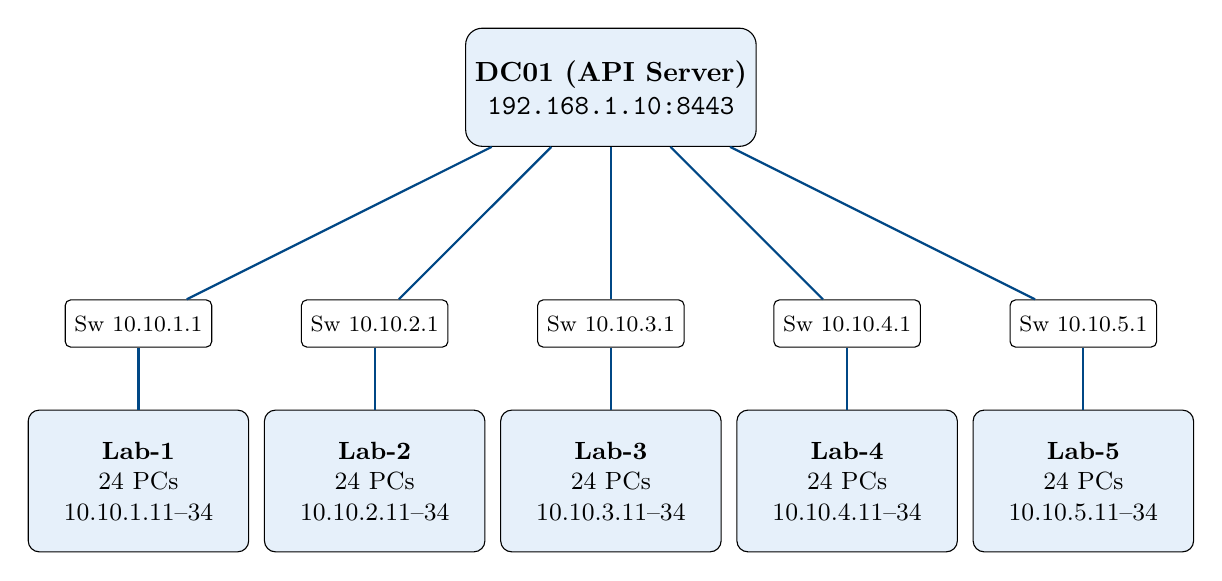
\begin{tikzpicture}[
    lab/.style={draw, rounded corners=4pt, fill=emislight, minimum width=2.8cm, minimum height=1.8cm, align=center, font=\small},
    sw/.style={draw, rounded corners=2pt, fill=white, minimum width=1.8cm, minimum height=0.6cm, align=center, font=\footnotesize},
    dc/.style={draw, rounded corners=6pt, fill=emislight, minimum width=3.5cm, minimum height=1.5cm, align=center},
    arrow/.style={thick, color=emisblue}
]
    % Core switch / DC
    \node[dc] (dcnode) at (0,3) {\textbf{DC01 (API Server)}\\\texttt{192.168.1.10:8443}};

    % Lab switches
    \node[sw] (sw1) at (-6,0) {Sw 10.10.1.1};
    \node[sw] (sw2) at (-3,0) {Sw 10.10.2.1};
    \node[sw] (sw3) at (0,0) {Sw 10.10.3.1};
    \node[sw] (sw4) at (3,0) {Sw 10.10.4.1};
    \node[sw] (sw5) at (6,0) {Sw 10.10.5.1};

    % Lab boxes
    \node[lab] (lab1) at (-6,-2) {\textbf{Lab-1}\\24 PCs\\10.10.1.11--34};
    \node[lab] (lab2) at (-3,-2) {\textbf{Lab-2}\\24 PCs\\10.10.2.11--34};
    \node[lab] (lab3) at (0,-2) {\textbf{Lab-3}\\24 PCs\\10.10.3.11--34};
    \node[lab] (lab4) at (3,-2) {\textbf{Lab-4}\\24 PCs\\10.10.4.11--34};
    \node[lab] (lab5) at (6,-2) {\textbf{Lab-5}\\24 PCs\\10.10.5.11--34};

    % Connections
    \draw[arrow] (dcnode) -- (sw1);
    \draw[arrow] (dcnode) -- (sw2);
    \draw[arrow] (dcnode) -- (sw3);
    \draw[arrow] (dcnode) -- (sw4);
    \draw[arrow] (dcnode) -- (sw5);
    \draw[arrow] (sw1) -- (lab1);
    \draw[arrow] (sw2) -- (lab2);
    \draw[arrow] (sw3) -- (lab3);
    \draw[arrow] (sw4) -- (lab4);
    \draw[arrow] (sw5) -- (lab5);
\end{tikzpicture}
\end{center}

\begin{tipbox}
All lab PCs must be domain-joined and have \textbf{WinRM} enabled (enabled by default via Group Policy on domain-joined machines). The API uses PowerShell Remoting to execute commands on PCs remotely --- no agent installation needed.
\end{tipbox}

\subsection{Enable WinRM on Lab PCs}

WinRM is usually enabled automatically on domain-joined PCs. If not, run this on each PC (or push via GPO):

\begin{lstlisting}
# On each lab PC (as admin)
Enable-PSRemoting -Force
Set-Item WSMan:\localhost\Client\TrustedHosts -Value "DC01" -Force
\end{lstlisting}

Or deploy via Group Policy:
\begin{enumerate}
    \item Open \textbf{Group Policy Management} $\rightarrow$ create GPO under \texttt{EMIS Computers}
    \item Navigate to: Computer Configuration $\rightarrow$ Policies $\rightarrow$ Administrative Templates $\rightarrow$ Windows Components $\rightarrow$ Windows Remote Management
    \item Enable \textbf{Allow remote server management through WinRM}
    \item Set IPv4 filter to \texttt{*}
\end{enumerate}

% ══════════════════════════════════════════════════════════════════════
\section{Lab PC Setup (120 Computers)}
% ══════════════════════════════════════════════════════════════════════

Every lab PC must be configured so that teachers and students can log in with their domain accounts, and the API server can manage them remotely.

\begin{warningbox}
\textbf{User data is isolated.} Each user gets a separate profile folder on the PC (\texttt{C:\textbackslash Users\textbackslash username\textbackslash}). Students cannot access each other's files. Only SuperAdmins (Domain Admins) can access all profiles. Files are stored locally on each PC's own disk --- the server does \textbf{not} share RAM or storage with lab PCs.
\end{warningbox}

\subsection{What Each PC Needs}

\begin{table}[H]
\centering
\begin{tabularx}{\textwidth}{c l X}
\toprule
\textbf{\#} & \textbf{Requirement} & \textbf{Details} \\
\midrule
1 & Windows 10/11 Pro or Education & Home edition cannot join a domain \\
2 & Static IP address & Each PC gets a fixed IP from its lab subnet (e.g., \texttt{10.10.1.11}) \\
3 & DNS pointing to DC & Primary DNS = \texttt{192.168.1.10} (the Domain Controller) \\
4 & Domain-joined & Joined to \texttt{emis.local} domain \\
5 & WinRM enabled & For remote management via the API \\
6 & Firewall rules & Allow WinRM (TCP 5985/5986) and ICMP ping from DC \\
\bottomrule
\end{tabularx}
\caption{Lab PC Requirements Checklist}
\end{table}

\begin{warningbox}
\textbf{Windows Home} edition cannot join a domain. All lab PCs must run Windows 10/11 \textbf{Pro}, \textbf{Enterprise}, or \textbf{Education}.
\end{warningbox}

\subsection{Step-by-Step PC Setup}

Repeat for each of the 120 PCs (or use a Windows deployment tool like WDS/MDT for imaging):

\subsubsection{1. Configure Static IP}

Set the IP based on the lab subnet. Example for Lab-1, PC \#5:

\begin{cmdbox}
\begin{tabular}{ll}
IP:      & \texttt{10.10.1.15} \\
Subnet:  & \texttt{255.255.255.0} \\
Gateway: & \texttt{10.10.1.1} \\
DNS 1:   & \texttt{192.168.1.10} (DC01) \\
DNS 2:   & \texttt{8.8.8.8} (fallback) \\
\end{tabular}
\end{cmdbox}

Or via PowerShell:

\begin{lstlisting}
# Set static IP (adjust InterfaceIndex, IP, gateway per PC)
$nic = Get-NetAdapter | Where-Object Status -eq "Up"
New-NetIPAddress -InterfaceIndex $nic.ifIndex -IPAddress "10.10.1.15" `
    -PrefixLength 24 -DefaultGateway "10.10.1.1"
Set-DnsClientServerAddress -InterfaceIndex $nic.ifIndex `
    -ServerAddresses "192.168.1.10","8.8.8.8"
\end{lstlisting}

\subsubsection{2. Join Domain}

\begin{lstlisting}
Add-Computer -DomainName "emis.local" -Restart
\end{lstlisting}

Enter \texttt{EMIS\textbackslash Administrator} credentials when prompted. PC reboots and is now domain-joined.

\subsubsection{3. Enable WinRM}

WinRM is usually auto-enabled on domain-joined PCs via Group Policy. Verify:

\begin{lstlisting}
# Check if WinRM is running
Get-Service WinRM

# If not enabled, run:
Enable-PSRemoting -Force
\end{lstlisting}

\subsubsection{4. Set Computer Name}

Use a consistent naming scheme: \texttt{LAB\{lab\#\}-PC\{number\}}

\begin{lstlisting}
# Example: Lab 2, PC 7
Rename-Computer -NewName "LAB2-PC07" -DomainCredential (Get-Credential) -Restart
\end{lstlisting}

\subsubsection{5. Verify from DC}

After setup, test from the Domain Controller:

\begin{lstlisting}
# Ping
Test-Connection -ComputerName LAB1-PC01 -Count 2

# Test WinRM
Test-WSMan -ComputerName LAB1-PC01

# Run remote command
Invoke-Command -ComputerName LAB1-PC01 -ScriptBlock { hostname }
\end{lstlisting}

\subsection{Bulk Setup with GPO}

Instead of configuring 400 PCs manually, use Group Policy to push settings automatically:

\begin{table}[H]
\centering
\begin{tabularx}{\textwidth}{l X}
\toprule
\textbf{GPO Setting} & \textbf{Path} \\
\midrule
Enable WinRM & Computer Config $\rightarrow$ Admin Templates $\rightarrow$ Windows Remote Management $\rightarrow$ Allow remote server management \\
Firewall: WinRM & Computer Config $\rightarrow$ Windows Settings $\rightarrow$ Security $\rightarrow$ Windows Firewall $\rightarrow$ Inbound Rules $\rightarrow$ Predefined: Windows Remote Management \\
Firewall: ICMP & Same path $\rightarrow$ Predefined: File and Printer Sharing (Echo Request) \\
Restrict local login & User Config $\rightarrow$ Admin Templates $\rightarrow$ Control Panel $\rightarrow$ limit Settings pages \\
\bottomrule
\end{tabularx}
\caption{GPO Settings for Lab PCs}
\end{table}

\subsection{Windows Deployment (Optional)}

For imaging 400 PCs efficiently:

\begin{enumerate}
    \item Install \textbf{Windows Deployment Services (WDS)} on a server
    \item Create a \textbf{reference image}: install Windows, join domain, enable WinRM, install standard software
    \item Capture the image with \textbf{Microsoft Deployment Toolkit (MDT)}
    \item PXE-boot each lab PC $\rightarrow$ select the image $\rightarrow$ auto-deploys in 15--20 minutes
    \item Use an \texttt{unattend.xml} answer file to auto-set hostname, IP, and domain join
\end{enumerate}

\begin{tipbox}
With MDT + WDS, you can deploy all 120 PCs in a single weekend. Each PC boots from the network, gets the image, joins the domain, and is ready for students and teachers.
\end{tipbox}

\subsection{What Teachers and Students Get}

Once a PC is set up, users log in with their domain credentials:

\begin{cmdbox}
\begin{tabular}{ll}
\textbf{Username:} & \texttt{EMIS\textbackslash suman.adhikari} \\
\textbf{Password:} & Their AD password (forced change on first login) \\
\end{tabular}
\end{cmdbox}

\begin{table}[H]
\centering
\begin{tabularx}{\textwidth}{l X X}
\toprule
\textbf{Feature} & \textbf{Teacher} & \textbf{Student} \\
\midrule
Login to any lab PC & \checkmark & \checkmark \\
Access shared drives (R/W) & \checkmark & \checkmark \\
Print (BW \& Color) & \checkmark & \checkmark \\
Internet (full, unrestricted) & \checkmark & \checkmark \\
Email \& LMS & \checkmark & \checkmark \\
Install software & --- (IT installs via API) & --- \\
\midrule
\multicolumn{3}{l}{\textbf{API-only features (not visible on the PC):}} \\
\midrule
View lab PC status via API & \checkmark (any lab) & --- \\
Reset student passwords via API & \checkmark & --- \\
Change own password via API & \checkmark & \checkmark \\
\bottomrule
\end{tabularx}
\caption{Teacher vs Student Capabilities on Lab PCs}
\end{table}

\begin{tipbox}
On the PC itself, teachers and students have the \textbf{exact same experience}. They log in with their AD credentials and use the PC normally. The only difference is what they can do through the \textbf{API} --- teachers can monitor labs and reset passwords, students can only change their own password.
\end{tipbox}

% ══════════════════════════════════════════════════════════════════════
\section{Verification}
% ══════════════════════════════════════════════════════════════════════

After running all three scripts, verify the deployment:

\subsection{Check Users}

\begin{lstlisting}
# Total users
Get-ADUser -Filter * | Measure-Object

# Students
Get-ADUser -Filter * -SearchBase "OU=Students,OU=EMIS Users,DC=emis,DC=local" | Measure-Object

# List first 10
Get-ADUser -Filter * -SearchBase "OU=EMIS Users,DC=emis,DC=local" -Properties Department |
    Select-Object -First 10 Name, SamAccountName, Department |
    Format-Table -AutoSize
\end{lstlisting}

\subsection{Check Groups}

\begin{lstlisting}
# List role groups
Get-ADGroup -Filter 'Name -like "Role-*"' | Select Name

# Count members
Get-ADGroupMember "Role-Students" | Measure-Object
Get-ADGroupMember "Role-Teacher" | Measure-Object
\end{lstlisting}

\subsection{Check OUs}

\begin{lstlisting}
Get-ADOrganizationalUnit -Filter * |
    Select Name, DistinguishedName |
    Format-Table -AutoSize
\end{lstlisting}

\subsection{GUI Tool}

Open \textbf{Active Directory Users and Computers}:

\begin{lstlisting}
dsa.msc
\end{lstlisting}

% ══════════════════════════════════════════════════════════════════════
\section{Join Client PC to Domain (Optional)}
% ══════════════════════════════════════════════════════════════════════

To test with a Windows 10/11 client VM:

\subsection{Create Client VM}

\begin{table}[H]
\centering
\begin{tabularx}{0.5\textwidth}{l X}
\toprule
\textbf{Setting} & \textbf{Value} \\
\midrule
Name    & Client-PC01 \\
OS      & Windows 10/11 64-bit \\
CPU     & 2 \\
RAM     & 2048 MB \\
Disk    & 40 GB \\
\bottomrule
\end{tabularx}
\end{table}

\subsection{Configure Client DNS}

\begin{warningbox}
The client's DNS \textbf{must} point to the Domain Controller's IP (\texttt{192.168.1.10}), not \texttt{8.8.8.8}. Without this, domain join will fail.
\end{warningbox}

\begin{cmdbox}
\begin{tabular}{ll}
IP:      & \texttt{192.168.1.20} \\
Subnet:  & \texttt{255.255.255.0} \\
Gateway: & \texttt{192.168.1.1} \\
DNS:     & \texttt{192.168.1.10} \\
\end{tabular}
\end{cmdbox}

\subsection{Join Domain}

\begin{lstlisting}
Add-Computer -DomainName "emis.local" -Restart
\end{lstlisting}

Enter domain admin credentials when prompted. After reboot, login as:

\begin{cmdbox}
\begin{tabular}{ll}
Username: & \texttt{EMIS\textbackslash suman.sharma} \\
Password: & \texttt{Welcome@123} (default --- will force change) \\
\end{tabular}
\end{cmdbox}

% ══════════════════════════════════════════════════════════════════════
\section{Network Diagram}
% ══════════════════════════════════════════════════════════════════════

\begin{center}
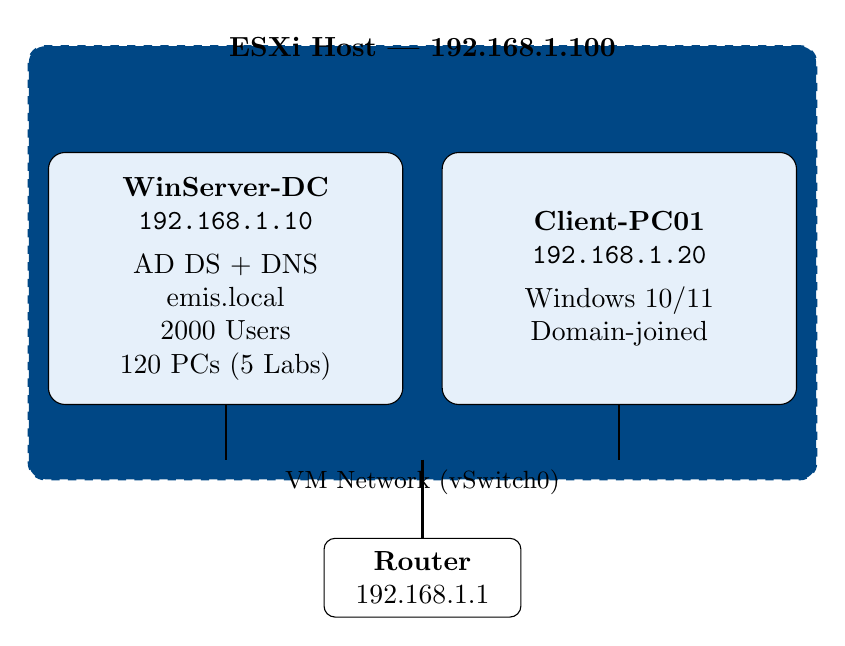
\begin{tikzpicture}[
    server/.style={draw, rounded corners=6pt, fill=emislight, minimum width=4.5cm, minimum height=3.2cm, align=center},
    host/.style={draw, rounded corners=6pt, fill=white, minimum width=10cm, minimum height=5.5cm, align=center, dashed, thick, color=emisblue},
    router/.style={draw, rounded corners=4pt, fill=white, minimum width=2.5cm, minimum height=1cm, align=center},
    label/.style={font=\small\ttfamily}
]
    % ESXi host
    \node[host] (esxi) at (0,0) {};
    \node[above] at (0,2.5) {\textbf{ESXi Host --- 192.168.1.100}};

    % VMs inside
    \node[server] (dc) at (-2.5,-0.2) {
        \textbf{WinServer-DC}\\
        \texttt{192.168.1.10}\\[4pt]
        AD DS + DNS\\
        emis.local\\
        2000 Users\\
        120 PCs (5 Labs)
    };
    \node[server] (client) at (2.5,-0.2) {
        \textbf{Client-PC01}\\
        \texttt{192.168.1.20}\\[4pt]
        Windows 10/11\\
        Domain-joined
    };

    % Network line
    \draw[thick, color=emisblue] (-5,-2.5) -- (5,-2.5);
    \node[below, font=\small] at (0,-2.5) {VM Network (vSwitch0)};

    % Connect VMs to network
    \draw[thick] (dc.south) -- (-2.5,-2.5);
    \draw[thick] (client.south) -- (2.5,-2.5);

    % Router
    \node[router] (router) at (0,-4) {\textbf{Router}\\192.168.1.1};
    \draw[thick] (0,-2.5) -- (router.north);
\end{tikzpicture}
\end{center}

% ══════════════════════════════════════════════════════════════════════
\section{Troubleshooting}
% ══════════════════════════════════════════════════════════════════════

\begin{longtable}{p{5cm} p{9.5cm}}
\toprule
\textbf{Problem} & \textbf{Solution} \\
\midrule
\endhead
VM can't boot from ISO & Check CD/DVD drive is connected and ``Connect at power on'' is checked \\[4pt]
Script says ``not recognized'' & Run \texttt{Set-ExecutionPolicy RemoteSigned -Force} first \\[4pt]
AD DS promotion fails & Ensure static IP and DNS (\texttt{127.0.0.1}) are set; server must ping the gateway \\[4pt]
Client can't join domain & Client's DNS \textbf{must} point to DC's IP (\texttt{192.168.1.10}), not \texttt{8.8.8.8} \\[4pt]
``Access Denied'' running scripts & Right-click PowerShell $\rightarrow$ ``Run as Administrator'' \\[4pt]
VM won't start (DVMT error) & Reduce video memory in VM settings to 8 MB \\[4pt]
API won't start (``No API keys'') & Run \texttt{.\textbackslash 04-AD-User-API.ps1 -GenerateKey} first to create at least one key \\[4pt]
Pode not found & Run \texttt{Install-Module -Name Pode -Force -Scope CurrentUser} \\[4pt]
PC shows offline in monitor & Check WinRM is enabled: \texttt{Test-WSMan -ComputerName LAB1-PC01} \\[4pt]
Cannot remote to lab PC & Ensure PC is domain-joined and WinRM firewall rule is open (TCP 5985/5986) \\[4pt]
API key rejected (403) & Verify the key in \texttt{api-keys.json} matches exactly; keys are case-sensitive \\
\bottomrule
\caption{Common Issues and Solutions}
\end{longtable}

% ══════════════════════════════════════════════════════════════════════
\section{Execution Summary}
% ══════════════════════════════════════════════════════════════════════

\begin{table}[H]
\centering
\begin{tabularx}{\textwidth}{c c X}
\toprule
\textbf{Order} & \textbf{Time} & \textbf{Action} \\
\midrule
1  & 10 min  & Download Windows Server 2019 ISO, upload to ESXi datastore \\
2  & 5 min   & Create VM (2 vCPU, 4 GB RAM, 60 GB disk) in ESXi \\
3  & 20 min  & Install Windows Server 2019 Desktop Experience \\
4  & 5 min   & Set static IP (192.168.1.10), DNS (127.0.0.1), hostname DC01 \\
5  & 5 min   & Run \texttt{01-Install-AD-DS.ps1} $\rightarrow$ server reboots \\
6  & 2 min   & Run \texttt{02-Create-RBAC-Structure.ps1} $\rightarrow$ OUs, groups, GPOs \\
7  & 10 min  & Run \texttt{03-Bulk-Create-Users.ps1 -GenerateSample} $\rightarrow$ 2000 users \\
8  & 5 min   & Edit \texttt{labs.json} with actual lab IPs, switches, PC hostnames \\
9  & 2 min   & Run \texttt{04-AD-User-API.ps1 -GenerateKey} $\rightarrow$ create service keys \\
10 & 1 min   & Run \texttt{04-AD-User-API.ps1} $\rightarrow$ API starts on port 8443 \\
11 & 5 min   & Verify with \texttt{dsa.msc}, join client PCs, test API endpoints \\
\bottomrule
\end{tabularx}
\caption{Step-by-Step Execution Order}
\end{table}

\vfill
\begin{center}
\textcolor{emisblue}{\rule{0.4\textwidth}{1pt}}\\[10pt]
{\small\textcolor{gray}{Prepared by EMIS IT Department --- June 2026}}\\
{\small\textcolor{gray}{Thapathali Campus, Institute of Engineering, Tribhuvan University}}
\end{center}

\end{document}
